% 附录 P：低温等离子体应用：从刻蚀到等离子体医学（v1.13.0 新增）
% 数值来源：tmp/appP_calc.py -> tmp/appP_calc.txt（正文与门禁的唯一来源）
% 单位口径：公式内的时间单位一律写 yr 与 day，避免中文字符落进数学字体
% 版权：只借鉴经典教材与文献的物理结论、公式形式与题型，文字与数值由本书自拟并独立复算
% 离线环境无法核验 DOI，故只给书名、作者、年份与卷页

第 2 章讲了碰撞与输运，第 11 章讲了鞘层与玻姆判据，附录 M 讲了加热与运行极限，附录 N 讲了聚变装置的边界与壁。这四块知识在\textbf{低温等离子体}（low-temperature plasma，$T_e\sim1$--$10\ \mathrm{eV}$、$T_{\mathrm{gas}}\approx300$--$400\ \mathrm{K}$）里汇成一条完全不同的应用链：把气体电离，用鞘层电场给离子定向，让离子带着能量去打表面，再让表面化学把能量换成刻蚀、沉积或活性分子。手机里的芯片、镀在玻璃上的薄膜、医院里的等离子体射流、臭氧发生器和尾气处理，都在这一条链上。

与相邻附录的分工：附录 J 回答"这个主题该读哪本书的哪一章"；附录 K 是完整解答的范例；附录 L 是自测题库；附录 M 是加热与运行极限的专题深挖；附录 N 是聚变装置的边界与壁；附录 O 是电推进。本附录换成\textbf{低温等离子体的工业与医疗应用}，并把每一笔能量、通量与速率都算成可以直接和手册对比的数。

\begin{tip}{单位与口径自查}{tip-appp-units}
本附录的数字都可以用计算器复算，仓库脚本 \texttt{appP\_calc.py} 列出了每一步。若结果差一个量级，先查三种口径错位：
\begin{enumerate}[nosep,leftmargin=1.6em]
  \item 密度与通量：$n_e$ 是 $\mathrm{m}^{-3}$ 还是 $\mathrm{cm}^{-3}$（差 $10^6$ 倍）？离子流密度常写成 $\mathrm{mA/cm^2}$，而 $1\ \mathrm{A/m^2}=0.1\ \mathrm{mA/cm^2}$；
  \item 温度：等离子体里的"温度"几乎都是能量单位 $\mathrm{eV}$，室温气体是 $0.0259\ \mathrm{eV}$，二者不能直接相加或相除——要先用 $1\ \mathrm{eV}=11600\ \mathrm{K}$ 换算；
  \item 气压：$\mathrm{Pa}$、$\mathrm{mTorr}$ 与 $\mathrm{Torr}$ 混用最常出错。本附录统一用 $1\ \mathrm{Torr}=133.322\ \mathrm{Pa}$，$1\ \mathrm{atm}=760\ \mathrm{Torr}$。帕申定律的自变量是 $p$ 与间隙 $d$ 的\textbf{乘积} $pd$（$\mathrm{Torr\cdot cm}$）。
\end{enumerate}
另：公式里的时间单位一律写作 \texttt{yr}（年）与 \texttt{day}（天），避免中文字符落进数学字体造成缺字。
\end{tip}

\section{三种放电与参数地图}
\label{sec:app-p-regimes}

低温等离子体不是一种东西，而是三种差别极大的工况。判据不是温度，而是\textbf{电离度}与\textbf{电子温度}：

\begin{itemize}[nosep,leftmargin=1.6em]
  \item 低气压放电（$0.1$--$100\ \mathrm{mTorr}$）：$n_e\sim10^{15}$--$10^{18}\ \mathrm{m}^{-3}$，电离度 $10^{-6}$--$10^{-3}$，$T_e=2$--$5\ \mathrm{eV}$。产业界的绝对主力——集成电路刻蚀、PECVD、溅射沉积都工作在这里。
  \item 大气压冷等离子体（$760\ \mathrm{Torr}$）：介质阻挡放电（DBD）与等离子体射流，能在开口环境下产生，不抽真空。医学、农业、表面改性靠它。
  \item 聚变边界等离子体（附录 N）：$T_e\approx15\ \mathrm{eV}$、$n_e\approx2\times10^{19}\ \mathrm{m}^{-3}$，比工业等离子体热得多也密得多，放在这张表里只作对照。
\end{itemize}

这张"参数地图"决定了后面所有数字的量级。由德拜长度与玻姆速度出发：

\begin{align}
  \lambda_D &= \sqrt{\frac{\epsilon_0 k_B T_e}{n_e e^2}}, \qquad c_s = \sqrt{\frac{k_B T_e}{m_i}}, \label{eq:app-p-debye}\\
  \Gamma_i &= n_e c_s, \qquad j_i = e\Gamma_i. \label{eq:app-p-flux}
\end{align}

其中玻姆速度里的温度要取 $T_e$（离子声速由电子压力驱动，见第 11 章）。表 \ref{tab:app-p-regimes} 用同一组公式算了五条工况。

\begin{table}[htbp]
  \centering
  \small
  \caption{五种等离子体工况的参数地图（$\lambda_D$ 与 $c_s$ 按式 \eqref{eq:app-p-debye}、$j_i$ 按式 \eqref{eq:app-p-flux}，氩离子）。第五行是附录 N 的聚变边界，用作对照。}
  \label{tab:app-p-regimes}
  \begin{tabular}{@{}lrrrrr@{}}
    \toprule
    工况 & $T_e\ (\mathrm{eV})$ & $n_e\ (\mathrm{m}^{-3})$ & $\lambda_D\ (\mathrm{\mu m})$ & $c_s\ (\mathrm{m/s})$ & $j_i\ (\mathrm{mA/cm^2})$ \\
    \midrule
    集成电路刻蚀（CCP/ICP） & 3.0 & $1.0\times10^{17}$ & 40.72 & 2692 & 4.313 \\
    溅射与 PECVD & 2.0 & $1.0\times10^{16}$ & 105.13 & 2198 & 0.352 \\
    等离子体医学（射流） & 1.5 & $1.0\times10^{19}$ & 2.88 & 1903 & 304.957 \\
    大气压 DBD 微放电通道 & 2.0 & $1.0\times10^{21}$ & 0.33 & 2198 & 35213.445 \\
    聚变边界（对照，附录 N） & 15.0 & $2.0\times10^{19}$ & 6.44 & 6019 & 1928.720 \\
    \bottomrule
  \end{tabular}
\end{table}

\textbf{刻蚀基准工况}：$T_e=3.0\ \mathrm{eV}$、$n_e=1.0\times10^{17}\ \mathrm{m}^{-3}$，得

\begin{equation}
  \lambda_D = 4.072\times10^{-5}\ \mathrm{m} = 40.72\ \mathrm{\mu m}, \quad
  c_s = 2692\ \mathrm{m/s}, \quad
  j_i = 4.313\ \mathrm{mA/cm^2}.
  \label{eq:app-p-etchbase}
\end{equation}

这两个数（$40\ \mathrm{\mu m}$ 的德拜长度、$4.3\ \mathrm{mA/cm^2}$ 的离子流）是后面所有刻蚀与沉积速率的输入。

\textbf{非平衡从哪来}：$T_e=3\ \mathrm{eV}$ 而 $T_{\mathrm{gas}}=0.0259\ \mathrm{eV}$（室温 $300\ \mathrm{K}$），

\begin{equation}
  \frac{T_e}{T_{\mathrm{gas}}} = \frac{3.0}{0.0259} \approx 116.
  \label{eq:app-p-noneq}
\end{equation}

\textbf{相差 116 倍}——这就是"低温等离子体"这个矛盾的名称的含义：电子热得能打断化学键，重粒子仍然是室温。原因很直白：电子质量小，在电场里被加速的速率 $\propto eE/m_e$ 是离子的 $\sqrt{m_i/m_e}\sim270$ 倍，而电子与重粒子碰撞的能量交换效率又 $\propto m_e/m_i$。等离子体由外场持续给电子注入能量，而重粒子只能通过碰撞慢慢"蹭"到一点。

\section{汤森雪崩与帕申定律}
\label{sec:app-p-paschen}

气体绝缘体只会因为一种正反馈而击穿：一个电子从电场里获得足够能量电离一个中性分子，产生的两个电子再各自电离，形成\emph{汤森雪崩}。汤森第一系数（每个电子每厘米产生的电离次数）为

\begin{equation}
  \alpha = A p \exp\!\left(-\frac{B p}{E}\right),
  \label{eq:app-p-townsend}
\end{equation}

其中 $p$ 是气压、$E$ 是电场，$A$ 与 $B$ 是气体常数。自持放电条件是雪崩产生的离子回到阴极后又能放出至少一个新的电子：

\begin{equation}
  \gamma\left(e^{\alpha d}-1\right) = 1
  \quad\Longrightarrow\quad
  \alpha d = \ln\!\left(1+\frac{1}{\gamma}\right) \equiv k.
  \label{eq:app-p-selfsustain}
\end{equation}

把式 \eqref{eq:app-p-townsend} 代入式 \eqref{eq:app-p-selfsustain}，解出击穿电压：

\begin{equation}
  V_b = \frac{B\,pd}{\ln(A\,pd)-k}, \qquad k = \ln\!\left(\ln\!\left(1+\frac{1}{\gamma}\right)\right).
  \label{eq:app-p-paschen}
\end{equation}

这就是\textbf{帕申定律}：$V_b$ 只依赖 $pd$ 的乘积，不依赖 $p$ 与 $d$ 各自是多少。

取空气的 $A=15\ \mathrm{/(cm\cdot Torr)}$、$B=365\ \mathrm{V/(cm\cdot Torr)}$、$\gamma=0.01$：

\begin{equation}
  k = \ln\!\left(\ln(1+1/0.01)\right) = 1.5293,
  \qquad
  V_{b,\min} = \frac{B\,pd_{\min}}{1}= 305.27\ \mathrm{V},
  \quad pd_{\min} = 0.8363\ \mathrm{Torr\cdot cm}.
  \label{eq:app-p-paschenmin}
\end{equation}

\begin{table}[htbp]
  \centering
  \small
  \caption{帕申曲线（$A=15$、$B=365$、$\gamma=0.01$）。最小值在 $pd=0.8363\ \mathrm{Torr\cdot cm}$ 处，$V_{b,\min}=305.27\ \mathrm{V}$；两侧都升高。}
  \label{tab:app-p-paschen}
  \begin{tabular}{@{}lrrrrrrr@{}}
    \toprule
    $pd\ (\mathrm{Torr\cdot cm})$ & 0.5 & 0.8363 & 1.0 & 2.0 & 5.0 & 10.0 & 76.0 \\
    \midrule
    $V_b\ (\mathrm{V})$ & 375.85 & 305.27 & 309.66 & 389.99 & 654.56 & 1048.46 & 5034.99 \\
    \bottomrule
  \end{tabular}
\end{table}

\textbf{最小值两侧的物理}：$pd$ 太小时，电子在到达阳极前来不及积累足够的电离碰撞次数，需要更高电压"补偿"；$pd$ 太大时，电子还没获得足够能量就先被弹性碰撞"冷却"，同样需要更高电压。这就是帕申曲线呈 V 形的原因（$1/pd$ 支与 $pd$ 支的竞争）。

\textbf{一个必须记住的陷阱}：大气压空气的间隙是 $1\ \mathrm{mm}$，则 $pd = 76\ \mathrm{Torr\cdot cm}$。把上面的公式照直外推，得到 $5035\ \mathrm{V}$。但大气压空气的经验击穿场强是

\begin{equation}
  E_{\mathrm{br}} = 3.0\times10^{6}\ \mathrm{V/m} = 30\ \mathrm{kV/cm},
  \label{eq:app-p-empirical}
\end{equation}

$1\ \mathrm{mm}$ 间隙只需 $3000\ \mathrm{V}$。外推值 $5035\ \mathrm{V}$ 是经验值的 $1.68$ 倍——\textbf{不能把低压帕申公式外推到大气压}。原因：$A$、$B$ 是在低 $E/p$ 区间标定的，大气压下的放电机制（空间电荷畸变、流注、光电离）已经不在汤森雪崩的框架内。

\textbf{大气压下的场强口径}：$1\ \mathrm{atm}$、$300\ \mathrm{K}$ 时

\begin{equation}
  N = \frac{p}{k_BT} = 2.4463\times10^{25}\ \mathrm{m}^{-3},
  \qquad
  \frac{E}{N} = \frac{3.0\times10^{6}}{2.4463\times10^{25}} = 1.2263\times10^{-19}\ \mathrm{V\cdot m^2} = 122.6\ \mathrm{Td},
  \label{eq:app-p-reducedfield}
\end{equation}

（$1\ \mathrm{Td} = 10^{-21}\ \mathrm{V\cdot m^2}$，以汤森命名）。约化场强 $E/N$ 是比 $E$ 本身更好的自变量：因为电子的能量增益与损失都正比于中性密度。在 $30\ \mathrm{kV/cm}$ 处，式 \eqref{eq:app-p-townsend} 给出 $\alpha = 1.0993\ \mathrm{cm^{-1}}$，于是 $\alpha d = 0.11$，远小于自持所需的 $k = 4.61$。

\textbf{这里出现一个看似矛盾的结果}：$\alpha d\ll k$，按式 \eqref{eq:app-p-selfsustain} 不该击穿，可经验上 $1\ \mathrm{mm}$ 间隙在 $3000\ \mathrm{V}$ 就击穿了。\textbf{这正是汤森理论在大气压下失效的标志}：$\alpha d<1$ 意味着平均每个初始电子产生的电离少于一次，雪崩无法自持；实际发生的是\emph{流注}（streamer）——局部空间电荷把电场畸变到远高于平均值，并且光电离提供了额外的种子电子。所以在大气压下，正确做法是承认经验值 $E_{\mathrm{br}}=30\ \mathrm{kV/cm}$，而不要用汤森公式反推。

\textbf{出处：} Raizer《Gas Discharge Physics》汤森雪崩与帕申定律章；Lieberman \& Lichtenberg《Principles of Plasma Discharges and Materials Processing》第 2 版第 1 章与第 14 章（帕申曲线与最小击穿电压）；本书第 2 章碰撞与电离。

\begin{figure}[htbp]
\centering
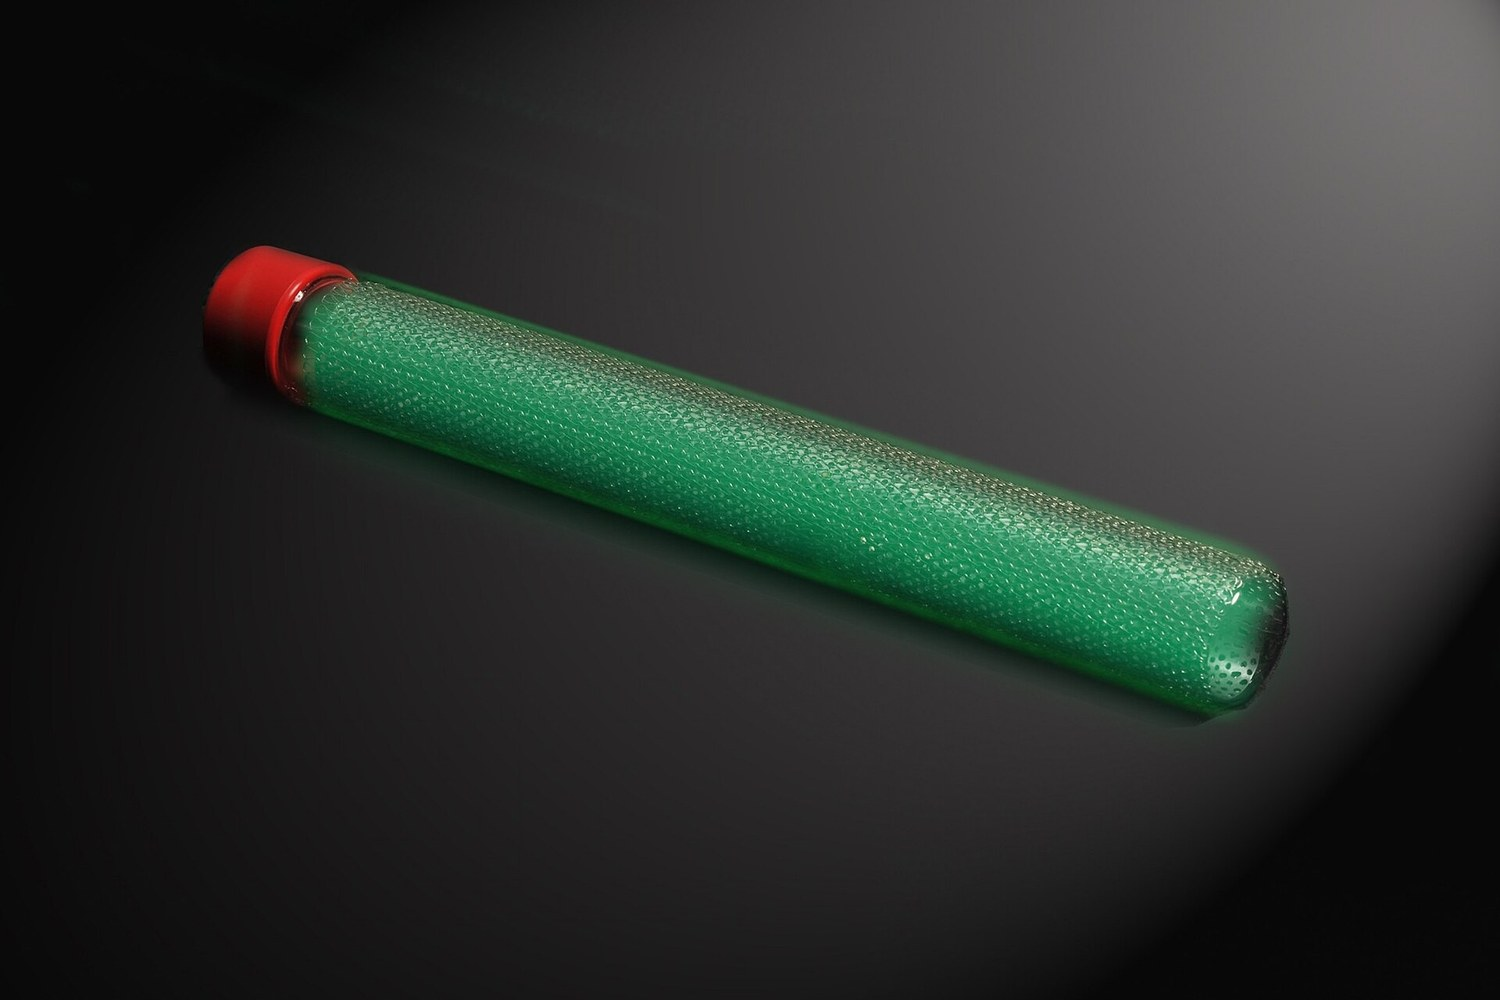
\includegraphics[width=0.78\textwidth]{../figures/p_corona_tube.jpg}
\caption{电晕放电管：大气压下的放电就长这样。介质阻挡放电把放电限制在介质表面附近，避免它收缩成弧；照片里这种电晕管是同一件事的另一种几何。}
\label{fig:photo-appp2}
\figsource{BentaxGermany，CC BY-SA 3.0（Wikimedia Commons）}
\end{figure}

\section{介质阻挡放电与大气压等离子体}
\label{sec:app-p-dbd}

要在开口环境里产生稳定放电，最容易的办法是在电极上盖一层介质。电荷积累在介质表面，把电场"抵消"掉，放电自己熄灭；交变电压反向后又重新点燃。这就是\textbf{介质阻挡放电}（DBD）。它天然是脉冲式的，每次只持续几十纳秒，正好避免了弧光化。

\textbf{电荷与功率账}：设介质厚度 $d=1\ \mathrm{mm}$、相对介电常数 $\epsilon_r=10$、面积 $A=100\ \mathrm{cm^2}$，介质电容为

\begin{equation}
  C_d = \frac{\epsilon_0\epsilon_r A}{d} = \frac{(8.854\times10^{-12})(10)(0.01)}{10^{-3}} = 8.854\times10^{-10}\ \mathrm{F} = 0.8854\ \mathrm{nF}.
  \label{eq:app-p-dbdcd}
\end{equation}

DBD 的功率不能用 $UI$ 算（电压电流有相位差），要用曼利（Manley）公式：

\begin{equation}
  P = 4 f C_d U_b \left(U_a - U_b\right),
  \label{eq:app-p-manley}
\end{equation}

其中 $U_a$ 是外加峰值电压、$U_b$ 是放电起始电压（气隙击穿后气隙上的电压基本被"钳"在这个水平）。

\begin{table}[htbp]
  \centering
  \small
  \caption{DBD 的电荷与功率账（$C_d=0.8854\ \mathrm{nF}$，$f=10\ \mathrm{kHz}$，$U_b=3000\ \mathrm{V}$，面积 $100\ \mathrm{cm^2}$）。功率按曼利公式 \eqref{eq:app-p-manley}。}
  \label{tab:app-p-dbd}
  \begin{tabular}{@{}lrrrr@{}}
    \toprule
    $U_a\ (\mathrm{V})$ & 半周期电荷 $(\mathrm{\mu C})$ & $P\ (\mathrm{W})$ & 功率密度 $(\mathrm{W/cm^2})$ & 每周期能量 $(\mathrm{mJ})$ \\
    \midrule
    4000 & 0.8854 & 106.3 & 1.063 & 10.63 \\
    5000 & 1.7708 & 212.5 & 2.125 & 21.25 \\
    \bottomrule
  \end{tabular}
\end{table}

注意 $U_a$ 从 $4000\ \mathrm{V}$ 提到 $5000\ \mathrm{V}$（只涨 25\%），功率从 $106.3\ \mathrm{W}$ 涨到 $212.5\ \mathrm{W}$（涨 100\%）——因为电荷 $\propto(U_a-U_b)$、而功率 $\propto U_b(U_a-U_b)$，$U_b$ 固定时功率对 $U_a$ 是线性的，两次之差被放大。

\textbf{微放电丝：非平衡的几何原因}。取 $U_a=4000\ \mathrm{V}$，每半周期约有 1000 根微放电丝（$10\ \mathrm{cm^{-2}}\times100\ \mathrm{cm^2}$），则单丝电荷

\begin{equation}
  q_{\mathrm{fil}} = \frac{0.8854\ \mathrm{\mu C}}{1000} = 0.885\ \mathrm{nC},
  \qquad
  \varepsilon_{\mathrm{fil}} = \frac{10.63\ \mathrm{mJ}}{2\times1000} = 5.3\ \mathrm{\mu J}.
  \label{eq:app-p-filament}
\end{equation}

若单丝持续 $\tau=10\ \mathrm{ns}$，峰值电流 $I=q/\tau = 0.0885\ \mathrm{A}$；丝半径取 $0.1\ \mathrm{mm}$（面积 $3.14\times10^{-8}\ \mathrm{m^2}$），丝内电流密度达 $2.818\times10^{6}\ \mathrm{A/m^2}=282\ \mathrm{A/cm^2}$。放电总体积取 $1.0\times10^{-5}\ \mathrm{m^3}$（$100\ \mathrm{cm^2}\times1\ \mathrm{mm}$），单丝体积

\begin{equation}
  V_{\mathrm{fil}} = \frac{4}{3}\pi (10^{-4})^3 = 4.189\times10^{-12}\ \mathrm{m^3},
  \label{eq:app-p-filvol}
\end{equation}

于是空间填充因子 $=4.189\times10^{-4}$、时间占空比 $=10\ \mathrm{ns}/100\ \mathrm{\mu s}=1.0\times10^{-4}$，两者相乘得

\begin{equation}
  f_{\mathrm{st}} = 4.189\times10^{-4}\times1.0\times10^{-4} = 4.189\times10^{-8}.
  \label{eq:app-p-fillfactor}
\end{equation}

\textbf{四千万分之一的时空体积}——能量只落在这极少数的丝里，因此重粒子气体温度仍停在 $300$--$400\ \mathrm{K}$，而电子在丝内被加热到几个 $\mathrm{eV}$。这就是大气压冷等离子体"宏观冷、微观热"的几何原因：不是能量不够，而是能量落得太集中、太快。

\textbf{出处：} Kogelschatz, \emph{Plasma Chemistry and Plasma Processing} \textbf{23}(1), 1--46 (2003)（DBD 综述与曼利公式）；Fridman, Chirokov \& Gutsol, \emph{Journal of Physics D} \textbf{38}, R1--R24 (2005)（大气压放电非平衡机制）；Raizer《Gas Discharge Physics》第 12 章。

\section{鞘层与离子轰击：刻蚀的方向性}
\label{sec:app-p-sheath}

等离子体加工的整个产业建立在一件事上：\textbf{让离子几乎垂直地砸向晶圆}。方向性来自鞘层——等离子体与所有表面之间必然出现的正电荷层（第 11 章）。

\textbf{鞘层厚度}由 Child 律给出（附录 K.7）：

\begin{equation}
  s = \frac{2}{3}\lambda_D\left(\frac{2V_s}{T_e}\right)^{3/4},
  \label{eq:app-p-child}
\end{equation}

其中 $V_s$ 是鞘层压降。取刻蚀基准 $T_e=3\ \mathrm{eV}$、$n_e=1\times10^{17}\ \mathrm{m}^{-3}$（$\lambda_D=40.72\ \mathrm{\mu m}$）：

\begin{equation}
  V_s = 100\ \mathrm{V}:\ s = 0.633\ \mathrm{mm}; \qquad
  V_s = 400\ \mathrm{V}:\ s = 1.791\ \mathrm{mm}.
  \label{eq:app-p-sheathnum}
\end{equation}

\textbf{方向性判据}。离子穿过鞘层时被加速到能量 $E_i\approx eV_s$，速度 $v_i=\sqrt{2E_i/m_i}$。但离子进入鞘层时带有横向热速度 $v_\perp\sim\sqrt{k_BT_e/m_i}$，于是入射角展宽

\begin{equation}
  \Delta\theta = \frac{v_\perp}{v_i} = \sqrt{\frac{T_e}{2V_s}}.
  \label{eq:app-p-angle}
\end{equation}

$V_s=100\ \mathrm{V}$ 时 $\Delta\theta = \sqrt{3/(2\times100)} = 0.1225\ \mathrm{rad} = 7.02^\circ$；$V_s=400\ \mathrm{V}$ 时降到 $3.51^\circ$。\textbf{提高偏压就能提高各向异性}——这是刻蚀设备往高偏压走的直接理由。同时注意

\begin{equation}
  s(100\ \mathrm{V}) = 0.633\ \mathrm{mm}
  \quad\text{而}\quad
  \lambda_{\mathrm{CX}} = 3.11\ \mathrm{mm}
  \ \ (\text{10 mTorr 氩气}),
  \label{eq:app-p-mfp}
\end{equation}

$\lambda/s = 4.91\gg1$：鞘层基本无碰撞（离子在鞘层内几乎不与中性粒子发生电荷交换），横向热运动没有被散射"抹匀"，方向性才得以保留。若气压升到几百 $\mathrm{mTorr}$，$\lambda$ 掉到 $\mathrm{\mu m}$ 量级，离子在鞘层里被多次散射，各向异性立刻崩掉——这是刻蚀必须工作在低气压的原因。

\textbf{刻蚀速率}。离子通量 $\Gamma_i = n_ec_s = 2.6918\times10^{20}\ \mathrm{m^{-2}s^{-1}}$，每个离子的溅射产额 $Y$（移走的硅原子数），则刻蚀速率

\begin{equation}
  R = \frac{Y\,\Gamma_i}{n_{\mathrm{Si}}},
  \qquad n_{\mathrm{Si}} = \frac{\rho_{\mathrm{Si}}}{m_{\mathrm{Si}}} = \frac{2329}{4.6637\times10^{-26}} = 4.9939\times10^{28}\ \mathrm{m^{-3}}.
  \label{eq:app-p-etchrate}
\end{equation}

\begin{table}[htbp]
  \centering
  \small
  \caption{刻蚀速率与选择比（$\Gamma_i=2.6918\times10^{20}\ \mathrm{m^{-2}s^{-1}}$，式 \eqref{eq:app-p-etchrate}）。物理溅射与反应离子刻蚀的差别全部体现在 $Y$ 上。}
  \label{tab:app-p-etch}
  \begin{tabular}{@{}lrrl@{}}
    \toprule
    过程 & $Y$ & 速率 $(\mathrm{nm/min})$ & 说明 \\
    \midrule
    物理溅射（纯氩） & 1.0 & 323.4 & 无化学辅助，边壁也被打 \\
    低产额情形 & 0.1 & 32.3 & 用于估算选择比下界 \\
    反应离子刻蚀（Si/Cl） & 1.2 & 388.1 & 化学与物理协同 \\
    \bottomrule
  \end{tabular}
\end{table}

\textbf{选择比}定义为两种材料刻蚀速率之比；在离子通量相同时它就等于产额之比 $1.2/0.1 = 12$。真实的反应离子刻蚀（RIE）选择比能到几十甚至上百，靠的是化学产额的差异而非物理溅射。

\textbf{出处：} Lieberman \& Lichtenberg《Principles of Plasma Discharges and Materials Processing》第 2 版第 6 章（鞘层）与第 15 章（刻蚀）；Child 1911、Langmuir 1913（Child--Langmuir 律原始文献，推导见附录 K.7）；本书第 11 章鞘层与玻姆判据。

\section{PECVD 与溅射沉积}
\label{sec:app-p-deposit}

刻蚀是把原子拿走，沉积是把原子放上去。两条路线的通量算法完全不同。

\textbf{PECVD（等离子体增强化学气相沉积）}：把硅烷（$\mathrm{SiH_4}$）送进放电，电子把它解离成 $\mathrm{SiH_3}$ 等自由基，自由基扩散到晶圆表面并沉积。给 20 sccm 硅烷、解离率 10\%：

\begin{align}
  \dot N_{\mathrm{SiH_4}} &= 20 \times 4.478\times10^{17} = 8.9559\times10^{18}\ \mathrm{s^{-1}}, \\
  \dot N_{\mathrm{Si}} &= 0.10\,\dot N_{\mathrm{SiH_4}} = 8.9559\times10^{17}\ \mathrm{s^{-1}}. \label{eq:app-p-sih4}
\end{align}

200 mm 晶圆面积 $A = \pi(0.1)^2 = 0.031416\ \mathrm{m^2}$，沉积通量 $2.8508\times10^{19}\ \mathrm{m^{-2}s^{-1}}$，生长速率

\begin{equation}
  R = \frac{2.8508\times10^{19}}{4.9939\times10^{28}} = 5.7085\times10^{-10}\ \mathrm{m/s} = 0.571\ \mathrm{nm/s} = 34.3\ \mathrm{nm/min}.
  \label{eq:app-p-pecvdrate}
\end{equation}

长 $1\ \mathrm{\mu m}$ 的膜需要

\begin{equation}
  t = \frac{10^{-6}}{5.7085\times10^{-10}} = 1751.8\ \mathrm{s} = 29.20\ \mathrm{min},
  \label{eq:app-p-pecvdtime}
\end{equation}

而送入的硅烷若 100\% 用上也需要同样的时间，故\textbf{硅烷利用率约 100\%}——这是"送进来的每一个硅原子都留下了"的理想上限；实际设备因排气与壁面沉积通常只有百分之几十，差额是工艺优化的主要空间。这正是 PECVD 比溅射快的原因：沉积速率不再由溅射产额决定，而由前驱体流量决定。

\textbf{溅射沉积}：靶面离子流密度 $J=100\ \mathrm{A/m^2}$，离子通量

\begin{equation}
  \Gamma_{\mathrm{ion}} = \frac{J}{e} = \frac{100}{1.602\times10^{-19}} = 6.2415\times10^{20}\ \mathrm{m^{-2}s^{-1}},
  \label{eq:app-p-sputflux}
\end{equation}

产额 $Y=0.5$ 时沉积速率 $374.9\ \mathrm{nm/min}$（同样按式 \eqref{eq:app-p-etchrate} 的形式）。它与刻蚀的公式形式相同、只是把"拿走"换成"放到衬底上"，代价是靶材被慢慢吃掉：

\begin{equation}
  I = 0.010\ \mathrm{A/cm^2}\times300\ \mathrm{cm^2} = 3.00\ \mathrm{A},
  \quad
  Q = I\,t = 3.00\times(100\times3600) = 1.0800\times10^{6}\ \mathrm{C},
  \label{eq:app-p-targetq}
\end{equation}

对应 $6.7408\times10^{24}$ 个离子；$Y=0.5$ 时移走 $3.37\times10^{24}$ 个铜原子，即 \textbf{355.6 g 铜}。连续 $100\ \mathrm{h}$（约 $4.2$ \texttt{day}）换 $356\ \mathrm{g}$ 靶材——这就是溅射靶的寿命账，与附录 N 的壁侵蚀是同一个物理（见 §\ref{sec:app-p-source} 的对照表）。

\textbf{出处：} Lieberman \& Lichtenberg《Principles of Plasma Discharges and Materials Processing》第 2 版第 15 章（PECVD 与溅射沉积）；Wasa、Kanno \& Kotera《Handbook of Sputter Deposition Technology》靶材与产额章；附录 N §N.4 溅射侵蚀。

\section{等离子体医学与农业：剂量学}
\label{sec:app-p-medicine}

等离子体医学的临床与农业研究每天都在用"剂量"这个词，但它和辐射剂量学不一样：这里必须同时给出\textbf{能量密度}和\textbf{活性物种密度}。

\textbf{能量剂量}。一支 1 W 的等离子体射流处理 $1\ \mathrm{cm^2}$ 处理 60 s：

\begin{equation}
  D = \frac{P\,t}{A} = \frac{1.0\times60}{1.0\times10^{-4}} = 6.0000\times10^{5}\ \mathrm{J/m^2} = 60.000\ \mathrm{J/cm^2}.
  \label{eq:app-p-dose}
\end{equation}

这是处理表面的总能量，但它几乎全部变成了热和紫外，只有极小一部分进了化学键。用液相化学产物可以把这个"极小一部分"量化：$100\ \mathrm{\mu M}$ 的 $\mathrm{H_2O_2}$ 溶液 $1\ \mathrm{mL}$ 含

\begin{equation}
  N = 100\times10^{-6}\times10^{-3}\times6.022\times10^{23} = 6.0221\times10^{16}
  \label{eq:app-p-h2o2num}
\end{equation}

个分子，把 60 J 平摊到这些分子上，每个分子分到 $9.9632\times10^{-16}\ \mathrm{J} = 6218.6\ \mathrm{eV}$。而 O--O 键能只有 $5.12\ \mathrm{eV}$，两者之比

\begin{equation}
  \frac{5.12}{6218.6} = 0.0823\%.
  \label{eq:app-p-medeff}
\end{equation}

\textbf{万分之八}。也就是说，即使我们把产出的过氧化氢全算成有用功，也只用掉了千分之一不到的电能；$99.9\%$ 以上变成了热、紫外和气流。这不是工艺缺陷，而是等离子体化学的固有代价：电子能量先被气体分子分掉，只有极小一撮落到我们想要的产物上。任何"等离子体医学效率"的讨论都必须从这个数字起步。

\textbf{固氮}。若放电把空气中的氮氧化成 NO，每个 NO 分子需要 $4.35\ \mathrm{eV}$，则

\begin{equation}
  \frac{4.35\times1.602\times10^{-19}\times6.022\times10^{23}}{10^{6}} = 0.42\ \mathrm{MJ/mol},
  \label{eq:app-p-no}
\end{equation}

$1\ \mathrm{kg}$ 氮对应 $71394.4\ \mathrm{mol}$ NO，故

\begin{equation}
  E = 71394.4\times0.42 = 29965.0\ \mathrm{MJ/kg\ N}.
  \label{eq:app-p-nfix}
\end{equation}

与哈伯法的 $\sim30\ \mathrm{MJ/kg}$ 相比，等离子体固氮的能耗高了\textbf{三个量级}。所以等离子体农业的现实定位不是"替代化肥"，而是现场、小规模、免高压免高温的补充手段（例如处理种子与灌溉水）。

\textbf{主导误差}：本节所有数字都是把总能量平摊到产物的口径，从它到真实的生物学剂量还差三步：射流出口到表面的距离（活性物种在气相里只有毫秒到秒的寿命）、气相湿度与液相体积（决定 $\mathrm{H_2O_2}$ 的生成与损失）、表面温升（几十 $\mathrm{K}$，会改变细胞响应）。所以文献里的剂量数只能当量级起点，不能跨装置直接比较。

\textbf{出处：} von Woedtke, Reuter, Masur \& Weltmann, \emph{Physics Reports} \textbf{530}, 291--320 (2013)（等离子体医学综述与剂量概念）；Graves, \emph{Journal of Physics D} \textbf{45}, 383001 (2012)（剂量学与活性物种）；Laroussi, \emph{IEEE Transactions on Plasma Science} \textbf{37}(6), 714--725 (2009)（射流与生物效应）。

\section{环境与催化：能量效率的硬账}
\label{sec:app-p-env}

低温等离子体在环保领域的卖点是"常温常压、随开随用"，但如果只讲卖点不讲电费，就无法判断它值不值得用。这一节把三种典型应用的电耗算成每分子 $\mathrm{eV}$。

\textbf{臭氧}。工业臭氧发生器的典型产率是 $100\ \mathrm{g/kWh}$（DBD 介质阻挡放电）。$1\ \mathrm{kWh}$ 产

\begin{equation}
  N = \frac{100}{47.9982}\times6.022\times10^{23} = 1.2547\times10^{24}
  \label{eq:app-p-o3num}
\end{equation}

个 $\mathrm{O_3}$ 分子，每个分子分摊 $2.8693\times10^{-18}\ \mathrm{J} = 17.91\ \mathrm{eV}$。而 $\mathrm{O_2}$ 的解离能只有 $5.12\ \mathrm{eV}$，理论极限效率

\begin{equation}
  \eta_{\max} = \frac{5.12}{17.91} = 28.6\%,
  \label{eq:app-p-o3eff}
\end{equation}

反过来说，产 $1\ \mathrm{kg}$ 臭氧至少要 $10.0\ \mathrm{kWh}$。这解释了为什么臭氧发生器总在拼"降低放电电压、提高微放电均匀性"——每一伏特都直接换成电费。

\textbf{VOC 降解}。取比能量输入 $\mathrm{SIE} = 300\ \mathrm{J/L}$（等离子体催化反应器的常见值），处理 $1000\ \mathrm{ppmv}$ 的甲苯：

\begin{equation}
  n = 1000\times10^{-6}\times2.6868\times10^{25}\times10^{-3} = 2.6868\times10^{19}\ \mathrm{L^{-1}},
  \label{eq:app-p-vocnum}
\end{equation}

每分子 $1.1166\times10^{-17}\ \mathrm{J} = 69.7\ \mathrm{eV}$。\textbf{关键在浓度}：同样的 SIE 若把浓度降到 $100\ \mathrm{ppmv}$，每分子的能量代价升到 $696.9\ \mathrm{eV}$——能量代价与浓度成反比。这是等离子体治理低浓度废气（如室内空气）的根本困难：你不得不用同样多的电去处理更少的分子。

\textbf{$\mathrm{CO_2}$ 解离}。$\mathrm{CO_2 \to CO + \frac12 O_2}$ 的吸热是 $2.9\ \mathrm{eV}$/分子，而等离子体的实际能耗常见 $10$--$100\ \mathrm{eV}$/分子，热力学效率只有 $3\%$--$29\%$。若用可再生电力驱动，即使按 $29\%$ 的上限，也意味着把三倍以上的绿电变成废热。

\begin{table}[htbp]
  \centering
  \small
  \caption{三种环境应用的能量效率硬账。每分子能耗与热力学最小能耗之比决定了效率上限。}
  \label{tab:app-p-env}
  \begin{tabular}{@{}lrrr@{}}
    \toprule
    应用 & 反应最小能耗 $(\mathrm{eV})$ & 实际每分子能耗 $(\mathrm{eV})$ & 效率上限 \\
    \midrule
    臭氧合成 & 5.12 & 17.91 & 28.6\% \\
    VOC 降解（甲苯 $1000\ \mathrm{ppmv}$） & --- & 69.7 & --- \\
    $\mathrm{CO_2}$ 解离 & 2.9 & 10--100 & 3\%--29\% \\
    \bottomrule
  \end{tabular}
\end{table}

\textbf{出处：} Kogelschatz, \emph{Plasma Chemistry and Plasma Processing} \textbf{23}(1), 1--46 (2003)（臭氧合成能量产率）；Kim, \emph{Plasma Processes and Polymers} \textbf{1}, 91--110 (2004)（等离子体催化与 VOC 处理）；Neyts, Ostrikov, Sunkara \& Bogaerts, \emph{Chemical Reviews} \textbf{115}, 13408--13446 (2015)（$\mathrm{CO_2}$ 与甲烷转化综述）；Attri, Ishikawa, Okumura, Koga \& Shiratani, \emph{Processes} \textbf{8}, 1002 (2020)（等离子体农业与活性物种）。

\section{六道估算练习}
\label{sec:app-p-problems}

答案都可以用仓库脚本 \texttt{appP\_calc.py} 复算，量级对上即算通过。

\textbf{练习 1（帕申与大气压）}。空气 $A=15\ \mathrm{/(cm\cdot Torr)}$、$B=365\ \mathrm{V/(cm\cdot Torr)}$、$\gamma=0.01$。(1) 求帕申最小值 $V_{b,\min}$ 与对应的 $pd$；(2) 若把公式外推到大气压 $1\ \mathrm{mm}$ 间隙（$pd=76\ \mathrm{Torr\cdot cm}$），得到多少伏？与实际经验值比较。

\textbf{解答}：$k=\ln(\ln(1+1/0.01))=1.5293$，$pd_{\min}=e^{k+1}/A = 0.8363\ \mathrm{Torr\cdot cm}$，$V_{b,\min}=B\,pd_{\min}=305.3\ \mathrm{V}$。外推 $pd=76$ 得 $5035\ \mathrm{V}$（脚本 \texttt{5034.99 V}），而大气压经验击穿场强 $30\ \mathrm{kV/cm}$ 给出 $1\ \mathrm{mm}$ 只需 $3000\ \mathrm{V}$：外推值是经验值的 $1.68$ 倍。结论：低压帕申公式不能外推，大气压必须用经验场强（式 \eqref{eq:app-p-empirical}）。

\textbf{练习 2（刻蚀速率与选择比）}。刻蚀基准工况 $T_e=3\ \mathrm{eV}$、$n_e=1\times10^{17}\ \mathrm{m}^{-3}$，硅原子密度 $n_{\mathrm{Si}}=4.9939\times10^{28}\ \mathrm{m}^{-3}$。设反应离子刻蚀的产额 $Y=1.2$、纯物理溅射 $Y=0.1$，求两者速率与选择比。

\textbf{解答}：$\Gamma_i=n_ec_s=2.6918\times10^{20}\ \mathrm{m^{-2}s^{-1}}$。按式 \eqref{eq:app-p-etchrate}，$Y=1.2$ 时

\begin{equation}
  R = \frac{1.2\times2.6918\times10^{20}}{4.9939\times10^{28}} \times60\times10^{9} = 388.1\ \mathrm{nm/min},
  \label{eq:app-p-ex2a}
\end{equation}

$Y=0.1$ 时 $32.3\ \mathrm{nm/min}$，选择比 $=1.2/0.1 = 12$。

\textbf{练习 3（鞘层厚度与方向性）}。同一基准工况，偏压 $V_s$ 取 $100\ \mathrm{V}$ 与 $400\ \mathrm{V}$。(1) 求鞘层厚度；(2) 求离子入射角展宽；(3) 已知 $10\ \mathrm{mTorr}$ 氩气的电荷交换平均自由程 $\lambda_{\mathrm{CX}}=3.11\ \mathrm{mm}$，判断鞘层是否无碰撞。

\textbf{解答}：由式 \eqref{eq:app-p-child}，$s = \frac23\lambda_D(2V_s/T_e)^{3/4}$。$V_s=100\ \mathrm{V}$：$s=0.633\ \mathrm{mm}$，$\Delta\theta=\sqrt{T_e/(2V_s)}=7.02^\circ$；$V_s=400\ \mathrm{V}$：$s=1.791\ \mathrm{mm}$，$\Delta\theta=3.51^\circ$。两者都满足 $s<\lambda_{\mathrm{CX}}=3.11\ \mathrm{mm}$（$\lambda/s=4.91>1$），鞘层基本无碰撞，方向性得以保留。

\textbf{练习 4（PECVD 生长 $1\ \mathrm{\mu m}$）}。20 sccm 硅烷，解离率 10\%，200 mm 晶圆。求沉积速率与长 $1\ \mathrm{\mu m}$ 所需时间，并说明硅烷利用率。

\textbf{解答}：$\dot N_{\mathrm{Si}}=8.9559\times10^{17}\ \mathrm{s^{-1}}$，$A=0.031416\ \mathrm{m^2}$，通量 $2.8508\times10^{19}\ \mathrm{m^{-2}s^{-1}}$，速率 $34.3\ \mathrm{nm/min}$，所需时间 $1751.8\ \mathrm{s}=29.2\ \mathrm{min}$。若按"送入的硅全部留下"计算，所需时间相同，故硅烷利用率 $100.0\%$（理想上限）。

\textbf{练习 5（臭氧电耗）}。臭氧产率 $100\ \mathrm{g/kWh}$，$\mathrm{O_2}$ 解离能 $5.12\ \mathrm{eV}$。(1) 求每分子分摊能量；(2) 求理论极限效率；(3) 求产 $1\ \mathrm{kg}$ 臭氧所需的电耗。

\textbf{解答}：$1\ \mathrm{kWh}=3.6\times10^{6}\ \mathrm{J}$ 产 $1.2547\times10^{24}$ 个分子，每分子 $2.8693\times10^{-18}\ \mathrm{J}=17.91\ \mathrm{eV}$。极限效率 $=5.12/17.91=28.6\%$。产 $1\ \mathrm{kg}$ 需要 $1000/100 = 10.0\ \mathrm{kWh}$。

\textbf{练习 6（医学剂量与固氮）}。一支 1 W 射流处理 $2\ \mathrm{cm^2}$ 共 60 s，求能量剂量；若放电把氮氧化成 NO（$4.35\ \mathrm{eV}$/分子），求每千克氮的能耗。

\textbf{解答}：总能量 $1.0\times60 = 60\ \mathrm{J}$，面积 $2\ \mathrm{cm^2}$，

\begin{equation}
  D = \frac{60}{2} = 30.0\ \mathrm{J/cm^2}.
  \label{eq:app-p-ex6a}
\end{equation}

固氮：$4.35\ \mathrm{eV}$/分子 $\to 0.42\ \mathrm{MJ/mol}$，$1\ \mathrm{kg}$ 氮 $=71394.4\ \mathrm{mol}$ NO，故 $29965.0\ \mathrm{MJ/kg\ N}$（哈伯法约 $30\ \mathrm{MJ/kg}$，差三个量级）。

\begin{tip}{先画能量链路，再算数}{tip-appp-chain}
本节六题有一个共同套路：\textbf{先写能量或粒子的守恒式，再代入数字}。例如刻蚀速率一定是"离子通量 $\times$ 产额 $\div$ 原子密度"，沉积速率一定是"前驱体通量 $\times$ 解离率 $\div$ 面积 $\div$ 原子密度"。凡是结果差一个量级，八成是漏了下列某一环：解离率 10\%、每分子电离耗能、面积用 $\mathrm{m^2}$ 还是 $\mathrm{cm^2}$、年产时间用 yr 还是实际放电时间。把每一环的因子写出来，比反复按计算器有用。
\end{tip}

\section{来源、分级与版权说明}
\label{sec:app-p-source}

本附录的做法与前几个附录一致：\textbf{只借鉴经典教材与文献的物理结论、公式形式与题型，文字、数值与表格全部由本书自拟并独立复算}。所有量级输入（$A=15$、$B=365$、$\gamma=0.01$、$\epsilon_r=10$、$\mathrm{SIE}=300\ \mathrm{J/L}$、产额 $Y$、离子流密度 $100\ \mathrm{A/m^2}$ 等）都在正文中显式写出，读者可以换掉任何一个重新算。

\begin{table}[htbp]
  \centering
  \small
  \caption{本附录各节的取材与本书的处理方式。}
  \label{tab:app-p-source}
  \begin{tabular}{@{}p{3.6cm}p{5.4cm}p{6.4cm}@{}}
    \toprule
    节 & 主要来源 & 本书处理 \\
    \midrule
    §P.1 参数地图 & Lieberman \& Lichtenberg 第 1 章 & 五工况自设，公式与量级取自教材 \\
    §P.2 帕申定律 & Raizer；Lieberman \& Lichtenberg 第 14 章 & 用 $A$、$B$、$\gamma$ 复算整条曲线与最小值 \\
    §P.3 DBD & Kogelschatz (2003)；Fridman 等 (2005) & 曼利公式与微放电丝账目自算 \\
    §P.4 鞘层刻蚀 & Lieberman \& Lichtenberg 第 6、15 章 & Child 律引用附录 K.7，速率用通量$\times$产额 \\
    §P.5 沉积 & Lieberman \& Lichtenberg 第 15 章；Wasa 等 & 前驱体流量法与靶侵蚀账目自算 \\
    §P.6 医学农业 & von Woedtke 等 (2013)；Graves (2012) & 剂量与活性物种双口径自算 \\
    §P.7 环境催化 & Kogelschatz (2003)；Kim (2004)；Neyts 等 (2015) & 每分子 $\mathrm{eV}$ 与效率上限自算 \\
    §P.8 六道练习 & 综合上列 & 题面与解答由本书自拟 \\
    \bottomrule
  \end{tabular}
\end{table}

\textbf{版权与独立性声明}：
\begin{itemize}[nosep,leftmargin=1.6em]
  \item 本附录\textbf{不复制}任何教材或论文的题目、解答、图表与数据表；
  \item 所有引用只到"书名/期刊名 + 作者 + 年份 + 卷页"一级，用于指路；
  \item 因离线环境无法核验 DOI，本附录\textbf{不写无法核实的 DOI 与卷页}的额外信息；
  \item 教材给出的量级（如臭氧产率 $100\ \mathrm{g/kWh}$、$\mathrm{SIE}=300\ \mathrm{J/L}$）在正文中显式标出，读者可替换；
  \item 所有数值均可用仓库脚本复算，与正文、门禁三方一致。
\end{itemize}

\begin{tip}{下一步读什么}{tip-appp-next}
建议先做附录 K.3（鞘层加速）与 K.7（Child--Langmuir 律），再读第 11 章鞘层与玻姆判据，然后做本附录六题。若对聚变方向的边界问题感兴趣，接着读附录 N（壁与偏滤器）；若对航天应用感兴趣，读附录 O（电推进）——§O.3 的空间电荷限制与本附录 §P.4 的鞘层是同一套 Child 律。
\end{tip}
